\icode{E-EXE-FI-L3-260625-002}
某实验小组欲制作一个两挡位（“\( \times 1\)”“\( \times 10\)”）的欧姆表，使用的实验器材如下：
  
\(A\).电流表\(G\)（满偏电流\(I_g =\) \,\qty{1}{mA}，内阻\(R_g =\) \,\qty{180}{\ohm}）；

\(B\).定值电阻\(R_0 =\) \,\qty{2}{\ohm}；
  
\(C\).定值电阻\(R_1 =\) \,\qty{18}{\ohm}；
  
\(D\).滑动变阻器\(R_2\)（最大阻值为\,\qty{1000}{\ohm}）；

\(E\).电源\(E\)（电动势为\,\qty{9}{V}）；
  
\(F\).单刀双挪开关\(S\)；
  
\(G\).红、黑表笔及导线若干。

其内部结构如图所示，回答下列问题：
  
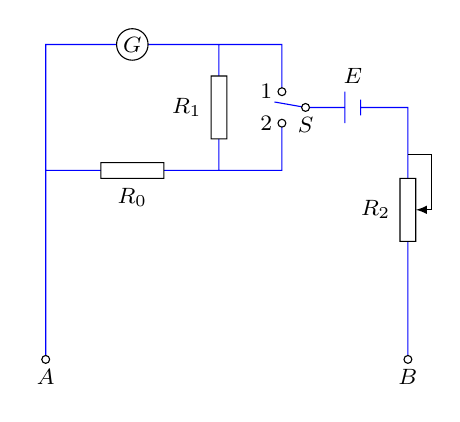
\begin{tikzpicture}[font=\footnotesize]
    \draw[blue] (0,-1)--(0,3)--(3,3)--(3,2.4) (0,1.4)--(3,1.4)--(3,2) (2.2,3)--(2.2,1.4) (3.8,2)--(3.8,2.4) (3.8,2.2)--(3.3,2.2)--++(170:.4) (4,2.1)--(4,2.3) (4,2.2)--(4.6,2.2)--(4.6,-1);
    \draw[fill=white] (1.1,3)node{\(G\)} circle(.2) (.7,1.3) rectangle(1.5,1.5) (2.1,2.6) rectangle(2.3,1.8) (4.5,1.3) rectangle(4.7,.5);
    \draw[fill=white] (0,-1)node[below]{\(A\)} circle(.05) (4.6,-1)node[below]{\(B\)} circle(0.05) (3,2.4)node[left]{\(1\)} circle(.05) (3,2)node[left]{\(2\)} circle(.05) (3.3,2.2)node[below]{\(S\)} circle(.05);
    \draw[-latex] (4.6,1.6)--(4.9,1.6)--(4.9,.9)--(4.7,.9);
    \node at(1.1,1.3)[below]{\(R_0\)};
    \node at(2.1,2.2)[left]{\(R_1\)};
    \node at(4.5,.9)[left]{\(R_2\)};
    \node at(3.9,2.6){\(E\)};
\end{tikzpicture}

（1）图中\(A\)接\underline{\hbox to 3em{}}（填“红”或“黑”）表笔；

（2）将单刀双掷开关\(S\)与1接通时，欧姆表的挡位为\underline{\hbox to 3em{}}（填“\( \times 1\)”或“\( \times 10\)”）；

（3）现用该欧姆表测量一未知电阻，选用“\( \times 10\)”挡位并欧姆调零后，将电阻接在\(A\)、\(B\)之间，发现电流表几乎满偏，断开电路并将“\( \times 10\)”挡位换成“\( \times 1\)”挡位，再次欧姆调零时，滑动变阻器的滑片\underline{\hbox to 3em{}}（填“向上”或“向下”）移动，使电流表满偏，再次将电阻接在\(A\)、\(B\)之间，稳定后电流表\(G\)的指针对准刻度盘上的\,\qty{0.6}{mA}处，则未知电阻\(R_{x} = \)\underline{\hbox to 3em{}}\,\qty{}{\ohm}。
\begin{answer}
    （1）黑（2）\( \times 10\)（3）向下\quad 60
\end{answer}